\documentclass[12pt, letter, leqno]{article}
\usepackage{times,tipa}
\usepackage{
    amsmath,
    amsthm,
    amssymb,
    mathtools,
    vowel,
    geometry,
    fancyhdr,
    arydshln,
    natbib,
    graphicx,
    xcolor,
    multicol,
    multirow,
    rotating,
    pstricks,
    colortab,
    booktabs,
    footnote,
    tablefootnote,
    tikz,
}
\usetikzlibrary{automata,positioning,arrows.meta}

\usepackage{caption}
\captionsetup{font=it,justification=centering}

\usepackage{multicol, multirow, endnotes, tree-dvips}

\renewcommand\floatpagefraction{.9}
\renewcommand\topfraction{.9}
\renewcommand\bottomfraction{.9}
\renewcommand\textfraction{.1}   
\setcounter{totalnumber}{50}
\setcounter{topnumber}{50}
\setcounter{bottomnumber}{50}

\raggedbottom

\usepackage[small,compact]{titlesec}

\usepackage[Symbolsmallscale]{upgreek} 

\titleformat*{\section}{\normalsize \bf}
\titleformat*{\subsection}{\normalsize \bf}
\titleformat*{\subsubsection}{\normalsize}
%
%\renewcommand{\footnotesize}{\normalsize}

\geometry{letterpaper, left=1in,right=1in,top=1in,bottom=1in}

\usepackage{setspace}
\doublespacing

\usepackage[singlelinecheck=off]{caption}


\usepackage{tree-dvips}

\usepackage{soul}

% \usepackage{gb4e}  % IMPORTANT: should be the last \usepackage
\usepackage{lingmacros}  % not to be confused with ling-macros

% bmatrix is a bit too big
% i packaged this out because it messed up my syntax highlighting
\newenvironment{setmatrix*}[1][c]
    {\renewcommand{\arraystretch}{0.6}
        \left\{%
        \begin{matrix*}[#1]}
    {\end{matrix*}\right\}}

\newenvironment{featmatrix*}[1][c]
    {\renewcommand{\arraystretch}{0.6}
        \left[%
        \begin{matrix*}[#1]}
    {\end{matrix*}\right]}


\frenchspacing

\newcommand{\sz}{\v}     

\newtheorem{theorem}{Theorem}
\newtheorem{definition}{Definition}

\begin{document}
        
\begin{center}
\textbf{
    Opaque Multi-tiered Strictly Local Maps in Chumash
}

Leo Peckham

\end{center}


% TODO: double check formatting instructions

\section{Introduction}

Long-distance harmony harmony is a rare, theoretically challenging phonological
process \citep{hansson01}. Rule-based theories require strangely defined
environments, and autosegmental theories take careful argument
\citep{jurgec11}; though optimality theory yields more success. However,
optimality theory suffers in situations where rules interact opaquely
\citep{mccarthy99}, where here opacity is as originally defined by
\citet[pg.~79]{kiparsky73a} (see Definition \ref{def:opacity}). Even the opacity
that optimality theory has been shown to handle can often require strong
machinery.

\begin{definition}
    A phonological rule $\mathbb{P}$ of the form $A \rightarrow B \big/ C
    \underline{\hspace{0.3cm}}~D$ is opaque if there are surface structures with
    either of the following characteristics:

    \begin{enumerate}
        \item instances of $A$ in the environment $C
            \underline{\hspace{0.3cm}}~D$; or
        \item instances of $B$ derived by $\mathbb{P}$ that occur in
            environments other than $C \underline{\hspace{0.3cm}}~D$.
    \end{enumerate}
\end{definition}\label{def:opacity}

Opaque long-distance harmony---like in Chumash, an isolate language indigenous
to California, compounds these factors---creates a vacuum and encourages new
tools and theories to gain strong intuition and make predictions.

In this paper I will apply the theory of output multi-tier strictly local
(OMTSL) maps, first described in \citet{burness&mcmullin19} to succinctly
explain Chumash's opaque sibilant harmony. I will then show that the standard
analysis of Chumash before being corrected by \citet{heinz&idsardi10} was never
possible under the OMTSL framework, and in fact belong to a wider class of
opaque patterns that it predicts not to exist in languages with long-distance
harmony.

\section{Background}\label{section:background-framework}

\citet{mcnaughton&papert71} introduced strictly local languages as a theory of
phonotactics, aiming to explain what types of well-formedness judgments can
exist in natural language. Many phonotactic patterns are strictly local, and
have seen a great deal of success theoretically, as well as achieving some
strong learnability results \citep{garcia+90,heinz10a,heinz10b,heinz&rogers13}.
Strict locality was extended to \textit{input} strict locality (ISL) and
\textit{output} strict locality (OSL) in \citet{chandlee14}, which provides a
much stronger formalism. An important property of ISL for this paper is that a
wide range of phonologically opaque maps are ISL \citep{chandlee+18}. Strictly
local languages, however, fail to account for long-distance dependencies.

Various ways to account for this deficiency have been proposed.
\citet{rogers+10} introduced strictly piecewise languages, which are also
efficiently learnable, but still fail to describe some long-distance patterns
\citep{cook84}. The strict locality hypothesis \citep{gafos99} simply suggests
that long-distance dependencies of this type simply do not exist, and are
really cases of feature spreading where the spread feature is imperceptible on
most segments. There is some phonetic evidence for this perspective
\citep{walker+09,gafos99}, but this hypothesis is contrary to \citet{hansson01}
and \citet{rose&walker04}, and there are issues with the learnability of
imperceptible features..

A stronger framework is that of tier-based strictly local languages
\citep{heinz+11}, based on the idea of the phonological tier
\citep{goldsmith76}. Phonological tiers are subsets of a phonological
inventory, usually arranged by some some natural class. For example, the vowel
tier of the Chumash word \textipa{/aSnisil/} `to tread' is \textipa{/aii/}.
Tier-based strictly local language languages keep all of the advantages of
strictly local languages (learnability, theoretical results), while also
succeeding in handling long-distance dependency more effectively
\citep{jardine&heinz16,burness&mcmullin19,mcmullin&hansson14,heinz+11}.

In much the same way that strict locality was extended to input and output
strict locality \citep{chandlee14}, \citet{burness&mcmullin19} extends
tier-based strict locality. In their paper, they describe output tier-based
strictly local functions, and note that input tier-based strictly functions
have a nearly identical construction.

Finally, \citet{burness&mcmullin20} introduce output mutli-tier strictly local
(OMTSL) functions. These resolve the inability tier-based strictly local
functions had to model more than one phonological process at a time in general.
In particular, OMTSL maps are the only strictly local framework currently able
to handle the opaque long-distance interactions I discuss in this paper. OMTSL
maps work by allowing a process to be predicated on more than one tier at a
time, but restricting the relations between tiers to avoid overgenerating.

To adhere to the existing literature, I choose to use the \textit{output}
multi-tier strictly local formalism instead of \textit{input} variant. This
also simplifies a few analyses later down the line, but there does not appear
to be a strict advantage of one over the other for managing long-distance
harmony.

\section{Mathematical preliminaries}

I will adopt standard the notation used for formal languages.

Let $\Sigma$ be an alphabet (set) of symbols. For the purposes of this paper,
$\Sigma$ will typically correspond one-to-one with out set of phonemes. I will
similarly use $\Delta$ as the set of phones. 

A string $w$ is a sequence of symbols in one of the two alphabets. If $w$ is a
sequence of symbols in $\Sigma$, it is an underlying representation; if $w$ is
a sequence of symbols in $\Delta$, it is a surface representation. A
formalization of intermediate representations is not necessary, since every map
used will be in a sense parallel. I will write $|w|$ to denote the length of
the string $w$. I write $\lambda$ to denote the empty string ($|\lambda| = 0$).

The Kleene star of an alphabet, $\Sigma^*$ or $\Delta^*$, denotes every
possible finite string generated by elements in the alphabet. Similarly
$\Sigma^k$ represents the set of every string of length $k$, and $\Sigma^{\le
k}$ represents the set of every string of length $k$ or smaller.

The phonology-phonetics interface can be viewed as a string-to-string function
$f : \Sigma^* \to \Delta^*$. I will denote the image of the set $S \subseteq
\Sigma^*$ under $f$ as $f(S)$, alongside usual function application.

Given two strings $u$ and $v$, I will denote their concatenation as $uv$. If
one of $u$ or $v$ is a set, this will denote the set of all strings in $u$ or
$v$ with $v$ concatenated as a suffix or $u$ concatenated as a prefix
respectively.

Beyond formal language theory, the remaining definitions and theorems are based
on from \citet{oncina&garcia92}, \citet{chandlee14}, \citet{chandlee+15},
\citet{burness&mcmullin19}, \citet{burness&mcmullin20}, and
\citet{burness&mcmullin21}. I will not use the formal descriptions in this
paper, but they are important to digest and have as reference. 

\begin{definition}
    The $k$-length suffix of a string, which I will denote as
    $\textnormal{suff}^k(w)$, is defined as the last $k$ symbols in the string
    $w$. If $|w| < k$, then the suffix is all of $w$.
\end{definition}

\begin{definition}
    The longest common prefix on a set of strings $S$, which I will denote as
    $\textnormal{lcp}(S)$, is the unique longest string $u$ with the property
    that for every $w \in S$, there exists some $x$ where $w = ux$. $u$ may be
    the empty string.
\end{definition}

\begin{definition}
    Given a function $f$, define its associated prefix function $f^p$ as:
    \[
        f^p(w) = \textnormal{lcp}(f(w\Sigma^*))
    \]
\end{definition}\label{def:fp}

These first three definitions are fairly simple string manipulation functions.
For Definition \ref{def:fp}, recall that $w\Sigma^*$ is the set of every string
prefixed by $w$.

\begin{definition}
    The tails of an input string $w$ with respect to some function $f$, which
    I will denote as $\textnormal{tails}_f(w)$, is defined by:
    \[
        \textnormal{tails}_f(w) = \{(y,v) \mid f(wy) = uv \wedge u =
        \textnormal{lcp}(f(w\Sigma^*))\}
    \]
\end{definition}

In words, the tails of a string $w$ is the pairing of every possible suffix $y$
to $w$, and the portion of $f(wy)$ that is a direct consequence of $y$.
Essentially, the tails of a string details how it must effect any possible
suffix. 

\begin{definition}
    The erasure function of a string with respect to some tier $T \subseteq
    \Sigma$, which I will denote as $\textnormal{erase}_T(w)$, is defined by:
    \[
        \textnormal{erase}_T(w) = \begin{cases*}
            \lambda & if $w = \lambda$ \\
            \textnormal{erase}_T(u) \sigma & if $w = u\sigma$ and $\sigma \in
            T$ \\
            \textnormal{erase}_T(u) & if $w = u\sigma$ and $\sigma \not\in T$

        \end{cases*}
    \]
    For convenience, I will write $\textnormal{suff}^k_T(w)$ to mean
    $\textnormal{suff}^k(\textnormal{erase}_T(w))$.
\end{definition}

The erasure function allows us to work with tiers in a straightforward way.
Consider the example from earlier: the vowel tier of \textipa{/aSnisil/} is
\textipa{/aii/}. To write this using erase, start by letting $T =
\{\text{\textipa{e,a,o,i,1,u}}\}$; then,
$\text{erase}_T(\text{\textipa{aSnisil}}) = \text{\textipa{aii}}$. 

I will now use the machinery defined above to outline several classes of
functions (maps). These maps are all additionally equivalent to classes of
formal languages and specific types of finite state machines.

\begin{definition}
    A function $f$ is $\text{OSL}_k$ if for all pairs of strings $u, v$ in
    $\Sigma^*$:
    \[
        \textnormal{suff}^{k-1}(f^p(u)) = \textnormal{suff}^{k-1}(f^p(v))
        \implies \textnormal{tails}_f(u) = \textnormal{tails}_f(v)
    \]
\end{definition}

The first class is the output strictly local (OSL) maps. Most classes that I
will use are defined in a similar way---partition the space of all input
strings by tail-equivalence under $f$ in the consequence, and then the function
is OSL if the partition is defined by a finite suffix of the outputs from the
class. Intuitively, a function is OSL if one can uniquely determine every
property of an output string that is meaningful to that function by
\textit{just} looking at the last few symbols of the output string.

OSL maps are fantastic at handling vowel harmony, where consonant cluster size
is bounded, and therefore so is $k$. They are not capable of handling
long-distance harmony, however, since there may be an arbitrary number of
segments between any two targets.

\begin{definition}
    A function $f$ is $\text{OTSL}_k$ if there is a tier $T \subseteq \Delta$ such that for all pairs of strings $u, v$ in $\Sigma^*$:
    \[
        \textnormal{suff}^{k-1}_T(f^p(u)) = \textnormal{suff}^{k-1}_T(f^p(v))
        \implies \textnormal{tails}_f(u) = \textnormal{tails}_f(v)
    \]
\end{definition}

Output tier-based strictly local (OTSL) functions works exactly the same as
output strictly local ones, except instead of the properties of the map being
predicated on \textit{whatever} the suffix of the string may be, it is only
predicated by those on the tier relevant to the process. This is exactly what
makes OTSL functions capable of handling long-distance harmony: they make the
arbitrarily many segments irrelevant to the process one is trying to describe
invisible, while keeping $k$ bounded.

\begin{definition}
    A function $f$ is $\text{OMTSL}_k$ if there is a finite set $\Theta$ of
    tiers $T \subseteq \Delta$ such that pairs of string for all $u, v$ in
    $\Sigma^*$:
    \[
        \left[\bigwedge_{T\in\Theta} \textnormal{suff}^{k-1}_T(f^p(u)) =
        \textnormal{suff}^{k-1}_T(f^p(v))\right] \implies
        \textnormal{tails}_f(u) = \textnormal{tails}_f(v)
    \]
    Additionally, for any pair of tiers $\tau_1, \tau_2$ in $\Theta$, either
    $\tau_1 \cap \tau_2 = \emptyset$ or $\tau_1 \subseteq \tau_2$.
\end{definition}

Finally, I define output multi-tier strictly local (OMTSL) functions. These are
additionally compatible with languages that have multiple harmony processes, or
have long-distance harmony that interacts with another process. They accomplish
this by allowing the tail-equivalence class to be predicated on multiple tiers.
For example, this allows long distance harmony to maintain its memory on one
tier without any arbitrary intervening segments, while allowing segments on
that tier to still undergo processes on other tiers. The partial ordering
enforced on tiers prevents pathological cases from greatly increasing the
complexity class of the maps.

It should be noted that all of these definitions only work on progressive
harmony, and imply a left-to-right directionality on the maps over in the
input/output strings. Indeed this is how \citet{chandlee14} defines OSL maps,
however, one can just as easily define right-to-left maps. In this paper, I
will directly use aspects of the left-to-right formalize on right-to-left maps,
since there is a simple way to translate between the two\footnote{
    %
    This binary is worth more investigation, either to try and resolve it in
    light of languages that have both progressive and regressive harmony, or to
    use it to predict that any given language will \textit{only} have one type.
    %
}. For more discussion of left-to-right maps and switching direction see
\citet{chandlee14} and \citet{heinz&lai13}.

\citep{chandlee14} and \citep{heinz&lai13} show how input strictly local
functions can be transformed to work on right-to-left processes as well. Since
the definitions are so similar I will only consider left-to-right processes in
this paper.

\begin{definition}
    The contribution of some segment $\sigma$ in $\Sigma$ relative to a string
    $w$ in $\Sigma^*$, with respect to a function $f$, denoted
    $\textnormal{cont}_f(\sigma, w)$ is defined by the relation:
    \[
        f^p(w) \textnormal{cont}_f(\sigma, w) = f^p(w\sigma)
    \]
\end{definition}

The contribution of a segment formalizes this notion dicussed above where the
visible effect on an output string is predicated by a segment in the input
string.

\section{Chumash}

Chumash, was an isolate language in California, now extinct. The language has
two main dialects of interest, the Inezeño dialect and the Ventureño dialect.
The first grammar of Chumash was \citeauthor{applegate72}'s
\citeyearpar{applegate72} thesis, based on Harrington's field notes on the
Inezeño dialect. A description of the Ventureño dialect was posthumously
published as \citet{harrington74}. The dialects are very similar, and most
papers on the language focus primarily on the Inezeño dialect. When I refer to
Chumash in the rest of this paper, I am referring to the Inezeño dialect.

\subsection{Applegate's Analysis}

Chumash features two interacting rules\footnote{
    %
    The $[\pm$anterior$]$ affricate pair \textipa{/ts/} and \textipa{/tS/}
    undergo the same rules, but there is more variation. I will not consider
    these phonemes for this paper.
    %
} that are important to this analysis: anterior dissimilation in
sibilant-dental clusters, and long-distance anterior harmony on its sibilants.

A brief consonant inventory of Chumash is presented in Table
\ref{tab:inventory}. There is also a contrastive plain-glottalized-aspirated
distinction on most segments, but no voice contrast. Chumash's vowel are
\textipa{/e,a,o,i,1,u/}.

\begin{table}[h]
    \centering
    \begin{tabular}{|l|cccccc|}
        \hline
        & Labial & Dental & Palatal & Velar & Uvular & Glottal \\
        \hline
        Nasals & m & n & & & & \\
        Stops & p & t & & k & q & \textipa{P} \\
        Affricates & & ts & \textipa{tS} & & & \\
        Fricatives & & s & \textipa{S} & x & & h \\
        Approximants & w & l & j & & & \\
        \hline
    \end{tabular}
    \caption{
        The Chumash consonant inventory. Modernized; based off
        \citet{applegate72}.
    }
    \label{tab:inventory}
\end{table}

\enumsentence{
    Dissimilation\label{ex:dissimilation} \citep[pp.~115,117]{applegate72}
    \vspace{-1em}
    \begin{tabbing}
        \hspace*{1em} \= \hspace*{6em} \= \hspace*{5em} \= \kill
        \>\textipa{/s+kal+w1j/} \> \textipa{[skaw'1j]}
            \> `he cuts a notch in it'\\
        \>\textipa{/s+tepuP/} \> \textipa{[StepuP]} \> `he gambles'\\
        \>\textipa{/s+niP/} \> \textipa{[SniP]} \> `his neck'\\
        \>\textipa{/s+lok'in/} \> \textipa{[Slok'in]} \> `he cuts it'
    \end{tabbing}
}

\enumsentence{
    Rule-based analysis of dissimilation \citep[pg.~118]{applegate72}
    \label{rule:dissimilation}
    \begin{multline*}
        \begin{featmatrix*}[l] 
            +\text{ant}\\
            +\text{cor}\\
            +\text{strid} 
        \end{featmatrix*}  
        %
        {\rightarrow} 
        %
        \begin{featmatrix*}[l] 
            -\text{ant}
        \end{featmatrix*} 
        \Big/
        \underline{\hspace{0.5cm}} 
        %
        {~+}
        \begin{featmatrix*}[l] 
            +\text{cons} \\
            +\text{ant} \\
            +\text{cor} \\
            +\text{strid}
        \end{featmatrix*} 
    \end{multline*}
}

The data in (\ref{ex:dissimilation}) shows the process of dissimilation in
Chumash, with the rule given in (\ref{rule:dissimilation}). Notably, Chumash
dissimilation only happens around morpheme
boundaries\footnote{\citet{applegate72} describes two different types of
morpheme boundaries in Chumash, close ($=$) and remove ($+$), but does not
distinguish between them for the present analysis.} \citep{applegate72}. For
the purposes of this paper, (\ref{rule:dissimilation}) is just
$\text{\textipa{s}} \rightarrow \text{\textipa{S}} \big/
\underline{\hspace{0.3cm}} {+} \{\text{\textipa{t, n, l}}\}$. Note that I do
not reanalyze this rule with $[+$continuant$]$ because of the affricates that
also undergo this rule (despite their strange status), and prefer to keep it
exactly as written in \citet{applegate72}.

The influence of morpheme boundaries in dissimilation was of particular
interest in previous analyses \citep{poser82,poser93,mccarthy07}, leading to
them using derived environment conditions. However, after correcting some
inaccuracies in the data, this process appears simpler than in the literature.
This will be discussed in more detail in Sections \ref{phm} and
\ref{section:opacity}.

\enumsentence{
    Harmony\label{ex:harmony} \citep[pp.~72,~119,~272]{applegate72}
    \vspace{-1em}
    \begin{tabbing}
        \hspace*{1em} \= \hspace*{10em} \= \hspace*{8em} \= \kill
        \>\textipa{/s+xalam+S/} \> \textipa{[SxalamS]} \> `it is wrapped'\\
        \>\textipa{/k+s1p1t+waS/} \> \textipa{[kS1p1twaS]}
            \> `I made acorn mush'\\
        \>\textipa{/waS+mas1x/}\footnote{$[+$anterior$]$ harmony seems to be
            much rarer than $[-$anterior$]$ harmony. Without a living native
            speaker, this is cause for concern, but ultimately I do not feel
            it affects the analysis.} \> \textipa{[wasmas1x]}
            \> `to be triple-ply'\\
        \>\textipa{/s+taja+nowon+waS/} \> \textipa{[StojonowonwaS]}
            \> `it stood upright'
    \end{tabbing}
}

\enumsentence{
    Rule-based analysis of harmony \citep[pg.~120]{applegate72}
    \label{rule:harmony}
    \begin{multline*}
        \begin{featmatrix*}[l] 
            +\text{cor}\\
            +\text{strid} 
        \end{featmatrix*}  
        %
        {\rightarrow} 
        %
        \begin{featmatrix*}[l] 
            \alpha\text{ant}
        \end{featmatrix*} 
        \Big/
        \underline{\hspace{0.5cm}} 
        %
        \begin{setmatrix*}[l] 
            C \\
            V \\
            +
        \end{setmatrix*}_0
        \begin{featmatrix*}[l] 
            \alpha\text{ant} \\
            +\text{cor} \\
            +\text{strid}
        \end{featmatrix*} 
    \end{multline*}
}

% TODO: actually, go back through that slideshow and just check off things

The harmony observed in (\ref{ex:harmony}) has been of particular interest in
the literature as an example of long-distance harmony. This type of harmony,
that can spread over morpheme boundaries and skip syllables, is rare
crosslinguistically \citep{hansson01}, and poses some big problems to popular
theories. It is neither strictly local nor input strictly local, and both
output strictly local and tier-based strictly local languages were in part
invented just to deal with patterns like these \citep{chandlee14,heinz+11}. 

\enumsentence{
    Dissimilation and harmony opacity\label{ex:interaction}
    \citep[pp.~119--120]{applegate72}
    \vspace{-1em}
    \begin{tabbing}
        \hspace*{1em} \= \hspace*{7em} \= \hspace*{5em} \= \kill
        \>\textipa{/s+uSla+s1q/} \> \textipa{[suslas1q]}
            \> `he presses it tight' \\
        \>\textipa{/s+is+t1P/} \> \textipa{[SiSt1P]} \> `he finds it' \\
        \>\textipa{/s+net+us/} \> \textipa{[snetus]} \> `he does it to him'
    \end{tabbing}
}

The data in (\ref{ex:interaction}) shows these rules interacting in a pattern
that is exactly \textit{fed counterfeeding on focus} (sometimes called a
\textit{Duke of York derivation}) \citep{bakovic11}. Fed counterfeeding on
focus occurs when a process changes some segment $A$ to $B$ in an environment
$C\_D$, and then another process changes it back again (see the full derivation
in (\ref{ex:fedcounterfeedingonfocus}). For the derivation in
(\ref{ex:fedcounterfeedingonfocus}) to work, dissimilation must be ordered
before harmony. Indeed, this is what \citet{applegate72} proposes, and it
explains the vast majority of the data. This opacity was even shown to be
productive, applying to loan-words \citep{applegate72}. However, there are also
a few known exceptions, given in (\ref{ex:noundergo}).

\enumsentence{
    Opaque fed counterfeeding on focus derivation of \textipa{/s+net+us/}.
    \label{ex:fedcounterfeedingonfocus}
    \vspace{-1em}
    \begin{tabbing}
        \hspace*{1em} \= \hspace*{4em} \= \kill

        \>\textipa{/s+net+us/} \> \\
        \>\textipa{Snetus} \> Dissimilation (feeds harmony) \\
        \>\textipa{snetus} \> Harmony (counterfeeds dissimilation) \\
        \>\textipa{[snetus]} \>
    \end{tabbing}
}

\enumsentence{
    Output of dissimilation does not undergo harmony\label{ex:noundergo}
    \citep[pg.~120]{applegate72}
    \vspace{-1em}
    \begin{tabbing}
        \hspace*{1em} \= \hspace*{8em} \= \hspace*{6em} \= \kill
        \>\textipa{/s+ti+jep+us/} \> \textipa{[Stijepus]} \> `he tells him' \\
        \>\textipa{/s+iS+lu+sisin/} \> \textipa{[SiSlusisin]}
            \> `they (dual) are grown awry'
    \end{tabbing}
}

\subsection{Poser, Hansson and McCarthy's analysis} \label{phm}

There have been several cumulative attempts made to justify the exceptions in
(\ref{ex:interaction}) by \citet{poser82,poser93,hansson01,mccarthy07}. I will
refer to this collective analysis as the Poser-Hansson-McCarthy (PHM) analysis.
This analysis revolves around trying to account for the supposed exceptions in
(\ref{ex:interaction}).

\enumsentence{
    Non-derived environment blocking in Finnish \citep{kiparsky73a,kiparsky93}
    \label{ex:finnish}
    \vspace{-1em}
    \begin{tabbing}
        \hspace*{1em} \= \hspace*{5em} \= \hspace*{4em} \= \kill
        \>\textipa{/\"aiti/} \> \textipa{[\"aiti]} \> `mother' \\
        \>\textipa{/vete/} \> \textipa{[vesi]} \> `water'
    \end{tabbing}
}

The PHM analysis tries to accomplish this by hypothesising that derived
environments block harmony. This is in a way dual to the opaque pattern of
non-derived environment blocking \linebreak\citep{bakovic11}, as can be seen in the
Finnish example in (\ref{ex:finnish}), so I will call this claimed opacity
\textit{derived environment blocking}. In the Finnish example, assibilation
($\text{\textipa{t}} \rightarrow \text{\textipa{s}} \big/
\underline{\hspace{0.3cm}} \text{\textipa{i}}$) only applies when \textipa{[i]}
was created by another rule (in this case word final raising). However, for
Chumash dissimilation to be an example of derived environment blocking, PHM
would need to explain the apparent under-application in words like
\textipa{/s+net+us/} $\rightarrow$ \textipa{[snetus]} from
(\ref{ex:interaction}). Fed counterfeeding examples like this are completely
left out of the PHM analysis, invalidating their argument for derived
environment blocking.

Furthermore, \citet{heinz&idsardi10} revealed through personal communication
with Applegate that instances like those in (\ref{ex:interaction}) are not
\textit{type} exceptions but rather \textit{token} exceptions. The token
exceptions are also rare, occurring less than 5\% of the time. This means that
in the majority of cases, the examples in (\ref{ex:interaction}) are realized
as \textipa{[stijepus]} and \textipa{[sislusisin]} respectively. There are many
ways to account for token variation like this\footnote{
    %
    Given the prevalence of morpheme boundary rules, and the distinction
    between close and remote morpheme boundaries, I hypothesize that the
    sibilant harmony variably gets blocked by close boundaries. That being
    said, any theory of variation is exceedingly hard to test without any
    living native speakers.
    %
}, but since this pattern is clearly not the rule, I will consider these
exceptions to be unattested for the sake of the analysis. This greatly
simplifies the analysis of Chumash, removing all effects of blocking and
reducing it to exactly what one would expect if dissimilation was ordered
before harmony. This is exactly what was originally claimed in Applegate's
analysis.

\section{OMTSL opacity}\label{section:opacity}

I would now like to show that by looking at Chumash through the lens of OMTSL
maps, the derived environment blocking opacity from the PHM analysis was never
possible in the first place. In fact, there are several types of long-distance
opacity that can arise in languages like Chumash that OMTSL maps predict to be
impossible. I will go over each of them in turn.

\subsection{Fed counterfeeding on focus} \label{section:dukeofyork}

I will consider two types of fed counterfeeding on focus corresponding two the
two rule orderings of harmony and dissimilation.

In the case where fed harmony counterfeeds dissimilation on focus, one simply
recovers Applegate's analysis, which was shown to be OMTSL in
\citet{burness&mcmullin20}.

If dissimilation were ordered before harmony, one would also get an example of
fed counterfeeding on focus. Consider the data in
(\ref{ex:dhfedcounterfeeding}) with the nonce word \textipa{/siSti+s/}.

\enumsentence{
    Fed dissimilation counterfeeds harmony on focus
    \label{ex:dhfedcounterfeeding}
    \vspace{-1em}
    \begin{tabbing}
        \hspace*{1em} \= \hspace*{4em} \= \kill

        \>\textipa{/siSti+s/} \> \\
        \>\textipa{sistis} \> Harmony \\
        \>\textipa{siStis} \> Dissimilation \\
        \>\textipa{[siStis]} \>
    \end{tabbing}
}

This is an example of fed counterfeeding on focus opacity that arises when
harmony is ordered before dissimilation. This can be viewed as if
\textipa{[St]} clusters, derived or not, are invisible to the process of
harmony; they will neither block harmony, nor undergo harmony.

By simply reversing the order of rule application, and despite causing the same
type of opacity, this pattern ceases to be OMTSL. To see why, consider that
there may be an arbitrary number of invisible clusters that surfaced between
the trigger and the target of an application of harmony. Since there is also
the requirement for \textipa{[S]} to be on the tier that harmony occurs, the
contribution of the trigger may be arbitrarily far away.

\subsection{Derived and non-derived environment blocking}

Next, I want to consider what derived and non-derived environment blocking
would look like in Chumash. In derived environment blocking (the PHM analysis),
only \textipa{[St]} sequences derived from dissimilation can block and trigger
harmony, and in non-derived environment blocking only morpheme internal
\textipa{[St]} sequences can block and trigger harmony. These are exact
opposites, and both are predicted to be impossible by OMTSL maps for the same
reason.

Consider again the nonce words \textipa{/siSti+s/} and \textipa{/sis+ti+s/}. In
either type of environment blocking, if one were to try to calculate the
contribution of the middle sibilant on the leftmost sibilant, they quickly find
that the contribution is dependent on the existence of a morpheme boundary
during dissimilation. Since there may be arbitrarily many \textipa{/+t/}
sequences between the leftmost sibilant and the long-distance middle sibilant,
it cannot be predicated on a derived environment condition without placing the
conditioning environment on the sibilant tier and causing a contradiction.
Therefore, neither type of environment blocking is OMTSL.

In general, it must be possible to calculate the contribution of a sibilant
without needing to remember how it arose. This implies that a categorical
blocking pattern would be OMTSL, and this is indeed true.

\subsection{Icy target blocking}

Introduced in \citet{jurgec11}, an \textit{icy target} is any target of harmony
that is itself a blocker. To see how this could look with (a modified) Chumash
phonology, consider the incorrect nonce word derivations in (\ref{ex:icy}).

\enumsentence{
    Icy target blocking in a modified Chumash
    \label{ex:icy}
    \vspace{-1em}
    \begin{tabbing}
        \hspace*{1em} \= \hspace*{6em} \= \hspace*{6em} \= \hspace*{5em}
            \= \kill

        \>\textipa{/Sis+ti+s/} \>\textipa{/SiSti+s/} \>\textipa{Sisti+s} \> \\
        \>\textipa{SiStis} \>\textipa{SiStis} \>-- \>Dissimilation \\
        \>\textipa{Sistis} \>\textipa{Sistis} \>\textipa{sistis}
            \> Harmony (\textipa{[St]} is icy)\\
        \>\textipa{[Sistis]} \>\textipa{[Sistis]} \>\textipa{[sistis]} \>
    \end{tabbing}
}

Like in environment blocking, this pattern is not OMTSL because the end result
of the leftmost sibilant is predicated on how the \textipa{[st]} cluster is
formed.

\subsection{Summary}

Compiling the results from this section arrives at Table \ref{tab:opacity}.

\begin{table}[h]
    \centering
    \begin{tabular}{ccccl} \toprule

        \textipa{/sis+ti+s/} & \textipa{/Sis+ti+s/} &
        \textipa{/siSti+s/} & \textipa{/SiSti+s/} &
        Type of Opacity \\
        
        \midrule

        \textipa{sistis} & \textipa{sistis} &
        \textipa{sistis} & \textipa{sistis} &
        Fed $H$ counterfeeds $D$ on focus (Applegate) \\

        \textipa{SiStis} & \textipa{SiStis} &
        \textipa{SiStis} & \textipa{SiStis} &
        Categorical blocking \\

        \midrule

        \textipa{siStis} & \textipa{siStis} &
        \textipa{siStis} & \textipa{siStis} &
        *Fed $D$ counterfeeds $H$ on focus\\

        \textipa{sistis} & \textipa{sistis} &
        \textipa{SiStis} & \textipa{SiStis} &
        *Non-derived environment blocking \\

        \textipa{SiStis} & \textipa{SiStis} &
        \textipa{sistis} & \textipa{sistis} &
        *Derived environment blocking (PHM) \\

        \textipa{sistis} & \textipa{Sistis} &
        \textipa{sistis} & \textipa{Sistis} &
        *Icy target \\

        \bottomrule

    \end{tabular}
    \caption{
        Possible types of opacity arising from the interaction between harmony
        ($H$) and dissimilation ($D$) in Chumash, seen in nonce-words. Rows 1-4
        are classified according to \citet{bakovic11}, and the interaction in
        row 5 is described in \citet{jurgec11}. * = impossible in OMTSL
        interpretations of Chumash\tablefootnote{
            %
            If these are ever attested in another language, it may be possible
            to account for them by augmenting OMTSL to be aware of autosegmental
            phonology \citep{goldsmith76}, and then using \textipa{\t{st}} and
            \textipa{\t{St}} as single segments on the harmony tier. This would
            require much more work, and may not be possible without also
            changing the complexity class.
            %
        }.
    }
    \label{tab:opacity}
\end{table}

It is clear that the only types of OMTSL long-distance harmony are the ones
where every column in the table is the same. This exactly corresponds to cases
where the long-distance harmony is not predicated on how the previous sibilant
came to be, keeping the harmony tier to just \textipa{\{s,S\}}.

\section{Discussion}

I hypothesize that the findings from the previous section are
cross-linguistically generalizable---all opaque interactions between a
long-distance process and a local process will either be fed counterfeeding on
focus where the long-distance process has priority, or the local process will
categorically block the long-distance process. I will argue that this is true
because OMTSL maps have several desirable properties that should hold for any
valid phonological theory. I will then discuss the consequences of this
hypothesis.

\subsection{Subregular predictions of OMTSL maps}

\begin{figure}[h]
    \centering
    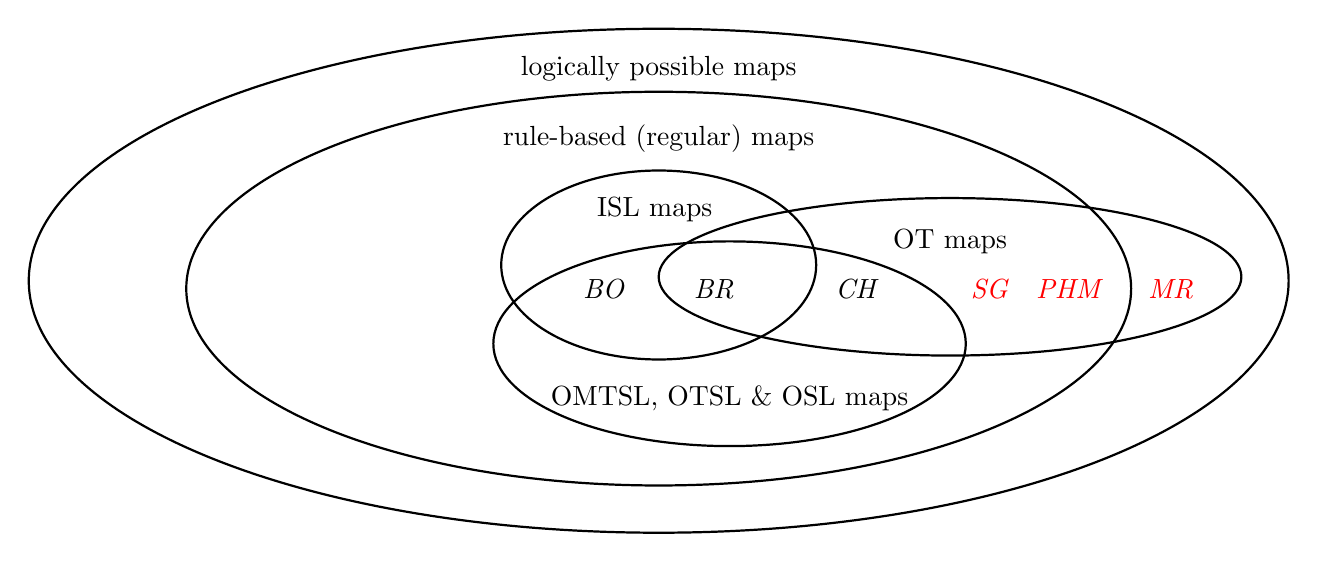
\begin{tikzpicture}[scale=1]

    \draw[thick] (0,-0.2) ellipse (8 and 3.2);
    \node at (0,2.5) {logically possible maps};

    \draw[thick] (0,-0.3) ellipse (6 and 2.5);
    \node at (0,1.6) {rule-based (regular) maps};

    \draw[thick] (0,0) ellipse (2 and 1.2);
    \node at (-0.05, 0.7) {ISL maps};

    \draw[thick] (3.7,-0.15) ellipse (3.7 and 1);
    \node at (3.7, 0.3) {OT maps};

    \draw[thick] (0.9,-1) ellipse (3 and 1.3);
    \node at (0.9, -1.7) {OMTSL, OTSL \& OSL maps};

    \node at (-0.7,-0.3) {\it BO};
    \node at (0.7, -0.3) {\it BR};
    \node at (2.5, -0.3) {\it CH};
    \node[color=red] at (4.2, -0.3) {\it SG};
    \node[color=red] at (5.2, -0.3) {\it PHM};
    \node[color=red] at (6.5, -0.3) {\it MR};

    \end{tikzpicture}
    \caption{
        Parts of the subregular hierarchy and their accompanying theories
        (regular text) as well as their predictions (italics) of different
        types of patterns. Unattested patterns are highlighted in red.
        (BO=Bedouin opacity; BR=Bedouin raising; CH=consonant harmony; SG=sour
        grapes harmony; PHM=Poser, Hansson and McCarthy's opacity (derived
        environment blocking); MR=majority rules harmony). See
        \citet{chandlee+18} and \citet{prickett22}.
    }
    \label{fig:hierarchy}
\end{figure}

The subregular hierarchy (shown in Figure \ref{fig:hierarchy}) generalizes the
complexities of various phonological maps in the same way the Chomsky hierarchy
generalizes the complexity of syntactic patterns. There is good reason to
believe that phonology is a subregular process. There are various regular maps
(like sour grapes harmony) that have never been attested and are not learnable
\citep{prickett22}, but are predicted to exist by several phonological
theories. There is also some experimental evidence supporting the subregular
hypothesis \citep{lai15,avcu18}.

Two extremely prevalent phonological theories, rule-based phonology and
optimality theory, are well known to fall outside the realm of subregular
languages, substantially overgenerating. This is a major failing of these
theories, since it is expected that a general theory of phonology can account
for every attested subregular pattern in phonology, and not a single unattested
pattern. Of course, this is infeasible to prove, but its reasonable to expect
that any phonological theory used to derive predictions will fit the current
understanding of attested phonological patterns.

One of the strongest justifications for strict locality is its ability to do
just this \citep{chandlee+18}. To account for consonant harmony, maps are
required to be output strictly local \citep{chandlee14} or tier strictly local
\citep{heinz+11}. However, both of these maps fail to account for Chumash
\citep{burness&mcmullin20}, which lands us exactly on OMTSL as being just
barely strong enough, exactly as desired.

Since OMTSL maps are strictly stronger than ISL maps, all of the opacity
results from \citep{chandlee+18} follow for free, firmly placing OMTSL maps as
a viable phonological theory for making general predictions.

\subsection{Learnability of OMTSL maps}

One of the motivating theories behind opacity comes from
\citeauthor{kiparsky73a}'s claim that opacity is difficult to learn, and the
consequences thereof. Despite this supposed difficulty, learners are still able
to acquire productive opacity without resorting to lexicalization
\citep{sanders03,ettlinger08}. \citet{bakovic11} provides a good treatment of
learnability in opacity, and why the relative learnability of opacity might not
be a strong notion.

All that being said, learnability of opaque maps remains an important topic in
the literature, so it is important that theories that account for opacity
provide strong learnability guarantees.

OMTSL functions have not yet been proven to be learnable in general without
additional restrictions \citep{burness&mcmullin21}, however there are good
theoretical and empirical reasons to believe that are.
\citet[pp.~147-154]{burness22} provides both a discussion of learnability in
OMTSL languages like Chumash, as well as results of an experiment on Chumash
data that prove Chumash's consonant harmony is learnable.

OMTSL maps also appear to hit a sweet spot with learnability.
\citet{prickett22} showed that sour grapes harmony is not learnable, which
falls just outside of the range of maps that are OMTSL.

\subsection{Why multiple tiers?}

Chumash (and other PHM opaque languages) is \textit{not} OTSL. To see this,
consider the (hypothetical) word \textipa{/sa+(ka+)$^*$s+ta/}. If the tier
consists of $\{$\textipa{s, S, t}$\}$, then one arrives at an incorrect guess
of the form \textipa{/Sa+(ka+)$^+$S+ta/}, so the morpheme boundary also needs
to be on the tier. However, if the morpheme boundary is included then there
could be an arbitrary number of morpheme boundary segments between the two
sibilants from the morpheme \textipa{/+ka+/}. This prevents Chumash from being
OTSL.

Another option would be to simply consider both dissimilation and harmony rules
independently, since they are each OTSL on their own. This does not work,
because to show that the opaque interaction is learnable, the entire language
(or subset of the language that creates the opaque interaction) is required to
be a single formalism with a learning guarantee. This is why OMTSL is needed
over OTSL.

Its also worth to consider that OMTSL maps being in a sense parallel is an
advantage for both neural computation and theory \citep{pruitt23}. The fact
that it can deftly address opacity while being parallel is a boon to the
theory.

\subsection{Consequences}

To be able to apply these findings more generally, it is useful to outline
exactly what is required for the opacity restrictions to apply.

\begin{enumerate}
    \item A long-distance process $\mathbb{A}$ acting on members of some tier
        $T$.
    \item A local process $\mathbb{B}$ acting on at least one member of $T$,
        but predicated on an environment disjoint from $T$.
    \item Evidence that both processes are productive.
\end{enumerate}

I predict that in any language that adheres to these conditions, $\mathbb{A}$
and $\mathbb{B}$ are guaranteed to interact opaquely. Additionally the
interaction will be one of: fed $\mathbb{A}$ counterfeeding $\mathbb{B}$ on
focus; or categorical blocking of $\mathbb{A}$ by any surface environment that
could be an output of $\mathbb{B}$.

As a next step, it would be very productive to review \citeauthor{hansson01}'s
\citeyear{hansson01} review of consonant harmony to confirm both the conditions
and predictions of the model. This review may also help explain the observation
that blocking in consonant harmony is exceedingly rare
\citep[pp.~213-214][pp.~486-487]{hansson01,rose&walker04}, since so many usual
blocking patterns are forbidden by an OMTSL framework in long-distance harmony.
 
I also put forward the suggestion to use OMTSL theory as a tool to analyze
other long-distance harmonic processes. For example, the blocking in Koyra
sibilant harmony \citep{hayward82,hayward86} is perfectly predicted by OMTSL.
Another example is Kalasha \citep{kochetov+21} sibilant harmony,
which while trivially analyzed using three tiers, could uncover valuable
insight on long-distance harmony by searching for a far neater single-tier OMTSL
analysis.

\section{Conclusion}


I showed that the theory of OMTSL maps succeeds as a general theory of
phonology, and is in particular useful for long-distance harmony and opacity. i
USED The theory corrects previous analyses of Chumash harmony, and predicts
that only two types of interactions are possible in languages with
long-distance harmony. These interactions are both opaque, and must be
independent of the conditioning environment of the local process. Further work
involves applying OMTSL maps to more cases of long-distance harmony.

\bibliography{bib}
\bibliographystyle{linquiry2}

\end{document}
